\documentclass{article}
\usepackage{tikz}
\usetikzlibrary{arrows}

% Language setting
% Replace `english' with e.g. `spanish' to change the document language
\usepackage[english]{babel}

% Set page size and margins
% Replace `letterpaper' with`a4paper' for UK/EU standard size
\usepackage[letterpaper,top=2cm,bottom=2cm,left=3cm,right=3cm,marginparwidth=1.75cm]{geometry}

% Useful packages
\usepackage{amsmath}
\usepackage{graphicx}
\usepackage[colorlinks=true, allcolors=blue]{hyperref}
\author{Roll no}
\title{Name} % Poster title
\date{}
\begin{document}

\maketitle

%Problem 1
\section*{Problem 1}

%Problem statement
Consider the graph on the right. Step through Dijkstra’s algorithm to find the Shortest Path from origin O to destination T. Show all steps.

\section*{Solution}

%Diagram Description
\textbf{Black = Visited\newline}
\textbf{white = Unvisited\newline}

%Graph
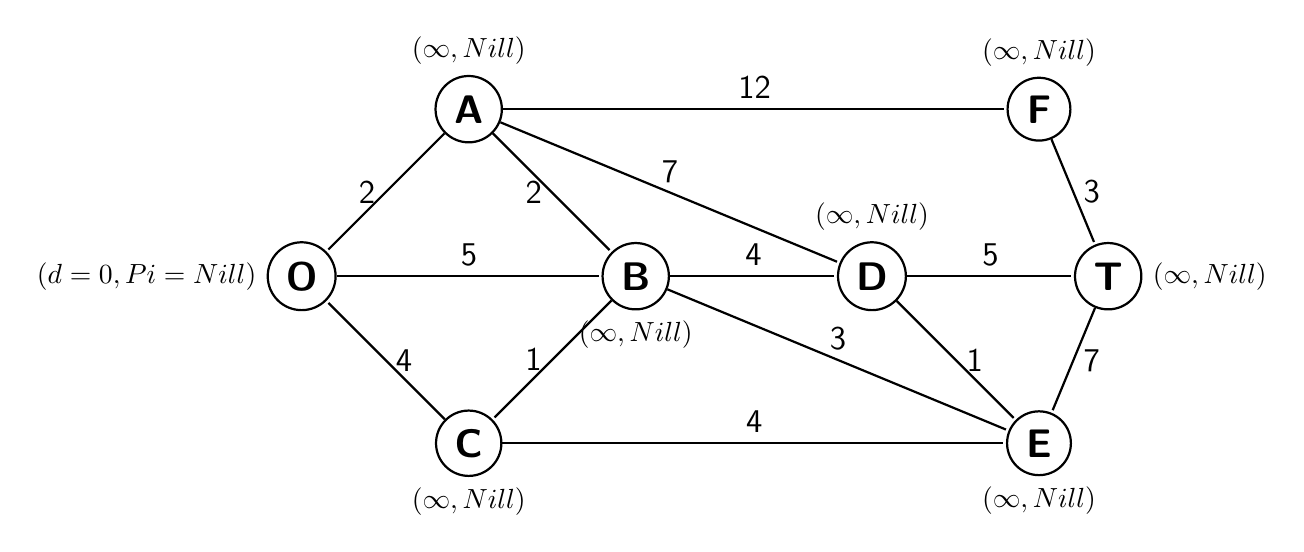
\begin{tikzpicture}[shorten >=1pt, auto, thick,
        node distance=3cm,
                    thick,main node/.style={circle,draw,font=\sffamily\Large\bfseries}]

%setting all nodes to infinity and Parents to Nill
  \node[main node, label=above:{$(\infty,Nill)$}] (1) {A};
  
%initilize starting node with 0 and parent to Nill
  \node[main node, label=left:{$(d=0,Pi=Nill)$}] (2) [below left of=1] {O};
  \node[main node, label=below:{$(\infty,Nill)$}] (3) [below right of=2] {C};
  \node[main node, label=below:{$(\infty,Nill)$}] (4) [below right of=1] {B};
  \node[main node, label=above:{$(\infty,Nill)$}] (6) [right of=4] {D};
  \node[main node, label=above:{$(\infty,Nill)$}] (5) [above right of=6] {F};
  \node[main node, label=right:{$(\infty,Nill)$}] (7) [right of=6] {T};
  \node[main node, label=below:{$(\infty,Nill)$}] (8) [below right of=6] {E};

  \path[every node/.style={font=\sffamily\large}]
    (1) edge node [left] {2} (4)
        edge [right] node[left] {2} (2)
        edge [right] node[above] {12} (5)
        edge [right] node[above] {7} (6)
    (2) edge node {5} (4)
    (3) edge node [right] {4} (2)
        edge [right] node[above] {4} (8)
    (4) edge node [left] {1} (3)
        edge [right] node[above] {4} (6)
        edge [right] node[above] {3} (8)
    (5) edge node [right] {3} (7)
    (6) edge node [right] {1} (8)
        edge [right] node[above] {5} (7)
    (7) edge node [right] {7} (8);
\end{tikzpicture}

%Dijsktra's Traversal Step 1
\subsection*{Step 1:\newline}

%Graph
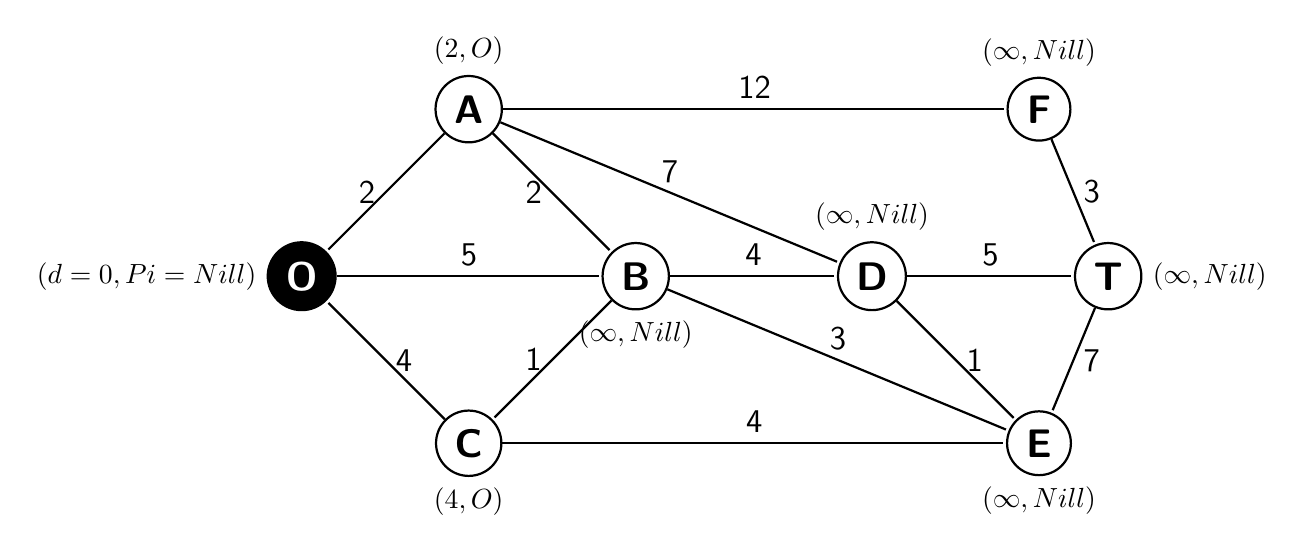
\begin{tikzpicture}[shorten >=1pt, auto, thick,
        node distance=3cm,
                    thick,main node/.style={circle,draw,font=\sffamily\Large\bfseries}]

  \node[main node, label=above:{$(2,O)$}] (1) {A};
  
% Turning node O to black representing that O is visited
  \node[main node, fill={rgb,1:red,0; green,0; blue,0}, text=white, draw=black, label=left:{$(d=0,Pi=Nill)$}] (2) [below left of=1] {O};
  
  %Setting distance of A and C by adding distance of O and edge weight
  \node[main node, label=below:{$(4,O)$}] (3) [below right of=2] {C};
  \node[main node, label=below:{$(\infty,Nill)$}] (4) [below right of=1] {B};
  \node[main node, label=above:{$(\infty,Nill)$}] (6) [right of=4] {D};
  \node[main node, label=above:{$(\infty,Nill)$}] (5) [above right of=6] {F};
  \node[main node, label=right:{$(\infty,Nill)$}] (7) [right of=6] {T};
  \node[main node, label=below:{$(\infty,Nill)$}] (8) [below right of=6] {E};

  \path[every node/.style={font=\sffamily\large}]
    (1) edge node [left] {2} (4)
        edge [right] node[left] {2} (2)
        edge [right] node[above] {12} (5)
        edge [right] node[above] {7} (6)
    (2) edge node {5} (4)
    (3) edge node [right] {4} (2)
        edge [right] node[above] {4} (8)
    (4) edge node [left] {1} (3)
        edge [right] node[above] {4} (6)
        edge [right] node[above] {3} (8)
    (5) edge node [right] {3} (7)
    (6) edge node [right] {1} (8)
        edge [right] node[above] {5} (7)
    (7) edge node [right] {7} (8);
\end{tikzpicture}


%Dijsktra's Traversal Step 2
\subsection*{Step 2:\newline}

%Graph
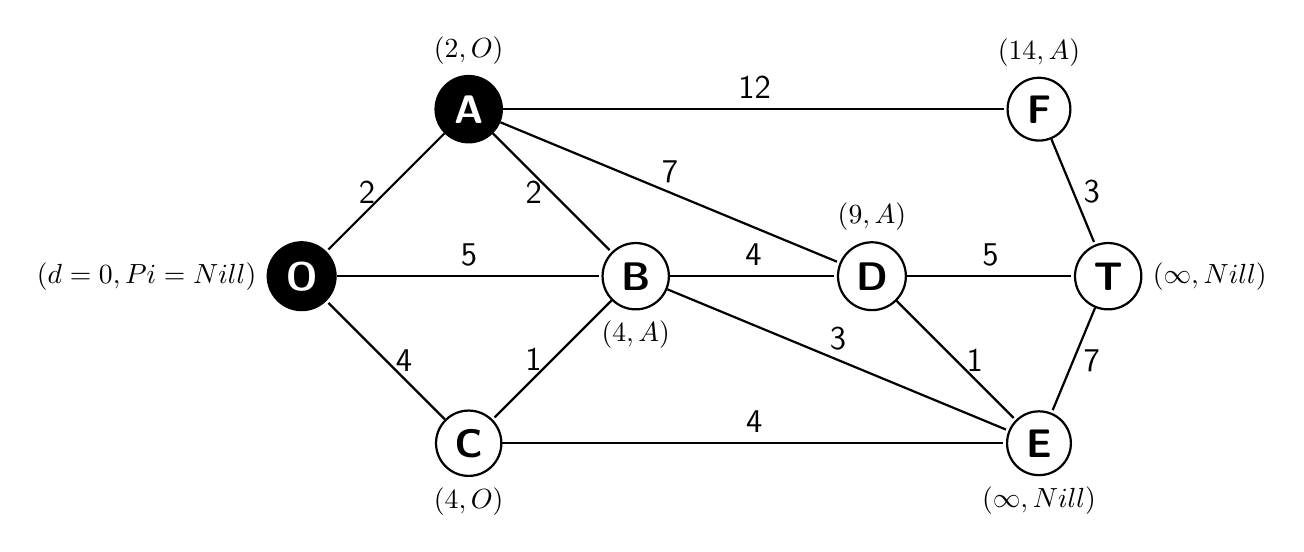
\begin{tikzpicture}[shorten >=1pt, auto, thick,
        node distance=3cm,
                    thick,main node/.style={circle,draw,font=\sffamily\Large\bfseries}]
                    
% Turning node A to black representing that A is visited
  \node[main node, fill={rgb,1:red,0; green,0; blue,0}, text=white, draw=black, label=above:{$(2,O)$}] (1) {A};
  \node[main node, fill={rgb,1:red,0; green,0; blue,0}, text=white, draw=black, label=left:{$(d=0,Pi=Nill)$}] (2) [below left of=1] {O};
  \node[main node, label=below:{$(4,O)$}] (3) [below right of=2] {C};

%Setting distance of B,F and D by adding distance of A and edge weight
  \node[main node, label=below:{$(4,A)$}] (4) [below right of=1] {B};
  \node[main node, label=above:{$(9,A)$}] (6) [right of=4] {D};
  \node[main node, label=above:{$(14,A)$}] (5) [above right of=6] {F};
  \node[main node, label=right:{$(\infty,Nill)$}] (7) [right of=6] {T};
  \node[main node, label=below:{$(\infty,Nill)$}] (8) [below right of=6] {E};

  \path[every node/.style={font=\sffamily\large}]
    (1) edge node [left] {2} (4)
        edge [right] node[left] {2} (2)
        edge [right] node[above] {12} (5)
        edge [right] node[above] {7} (6)
    (2) edge node {5} (4)
    (3) edge node [right] {4} (2)
        edge [right] node[above] {4} (8)
    (4) edge node [left] {1} (3)
        edge [right] node[above] {4} (6)
        edge [right] node[above] {3} (8)
    (5) edge node [right] {3} (7)
    (6) edge node [right] {1} (8)
        edge [right] node[above] {5} (7)
    (7) edge node [right] {7} (8);
\end{tikzpicture}


%Dijsktra's Traversal Step 3
\subsection*{Step 3:\newline}

%Graph
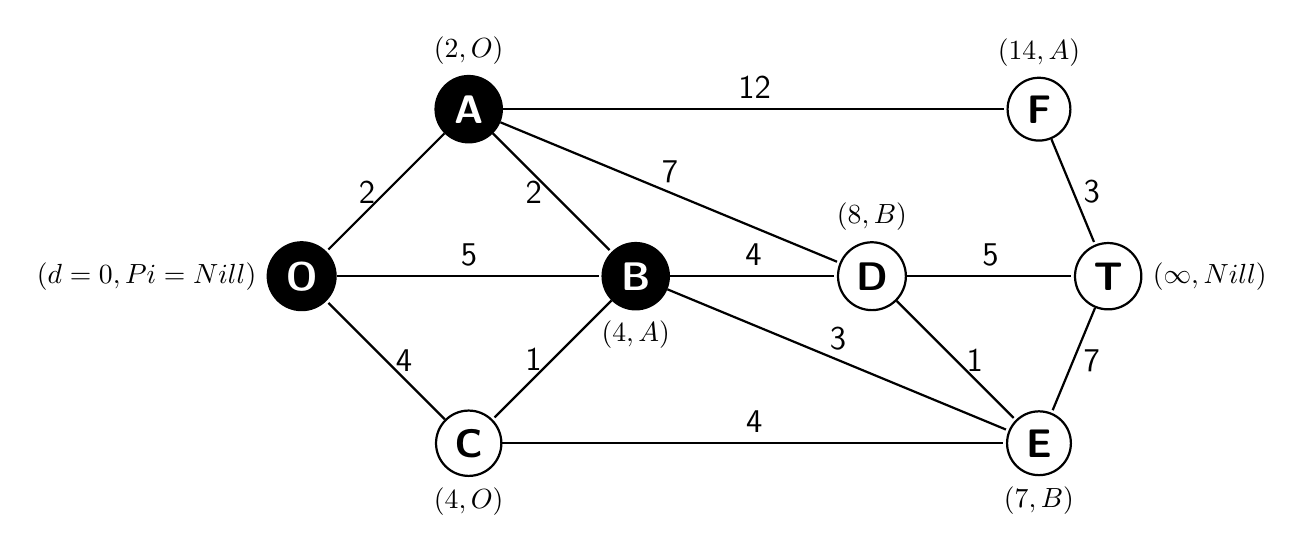
\begin{tikzpicture}[shorten >=1pt, auto, thick,
        node distance=3cm,
                    thick,main node/.style={circle,draw,font=\sffamily\Large\bfseries}]
                    

  \node[main node, fill={rgb,1:red,0; green,0; blue,0}, text=white, draw=black, label=above:{$(2,O)$}] (1) {A};
  \node[main node, fill={rgb,1:red,0; green,0; blue,0}, text=white, draw=black, label=left:{$(d=0,Pi=Nill)$}] (2) [below left of=1] {O};

  %C distance not updated because it is already less than B's node + edge
  \node[main node, label=below:{$(4,O)$}] (3) [below right of=2] {C};

% Turning node B to black representing that B is visited
  \node[main node, fill={rgb,1:red,0; green,0; blue,0}, text=white, draw=black, label=below:{$(4,A)$}] (4) [below right of=1] {B};
  
  %Setting distance of D and E by adding distance of B and edge weight
  \node[main node, label=above:{$(8,B)$}] (6) [right of=4] {D};
  \node[main node, label=above:{$(14,A)$}] (5) [above right of=6] {F};
  \node[main node, label=right:{$(\infty,Nill)$}] (7) [right of=6] {T};
  \node[main node, label=below:{$(7,B)$}] (8) [below right of=6] {E};

  \path[every node/.style={font=\sffamily\large}]
    (1) edge node [left] {2} (4)
        edge [right] node[left] {2} (2)
        edge [right] node[above] {12} (5)
        edge [right] node[above] {7} (6)
    (2) edge node {5} (4)
    (3) edge node [right] {4} (2)
        edge [right] node[above] {4} (8)
    (4) edge node [left] {1} (3)
        edge [right] node[above] {4} (6)
        edge [right] node[above] {3} (8)
    (5) edge node [right] {3} (7)
    (6) edge node [right] {1} (8)
        edge [right] node[above] {5} (7)
    (7) edge node [right] {7} (8);
\end{tikzpicture}



%Dijsktra's Traversal Step 4
\subsection*{Step 4:\newline}

%Graph
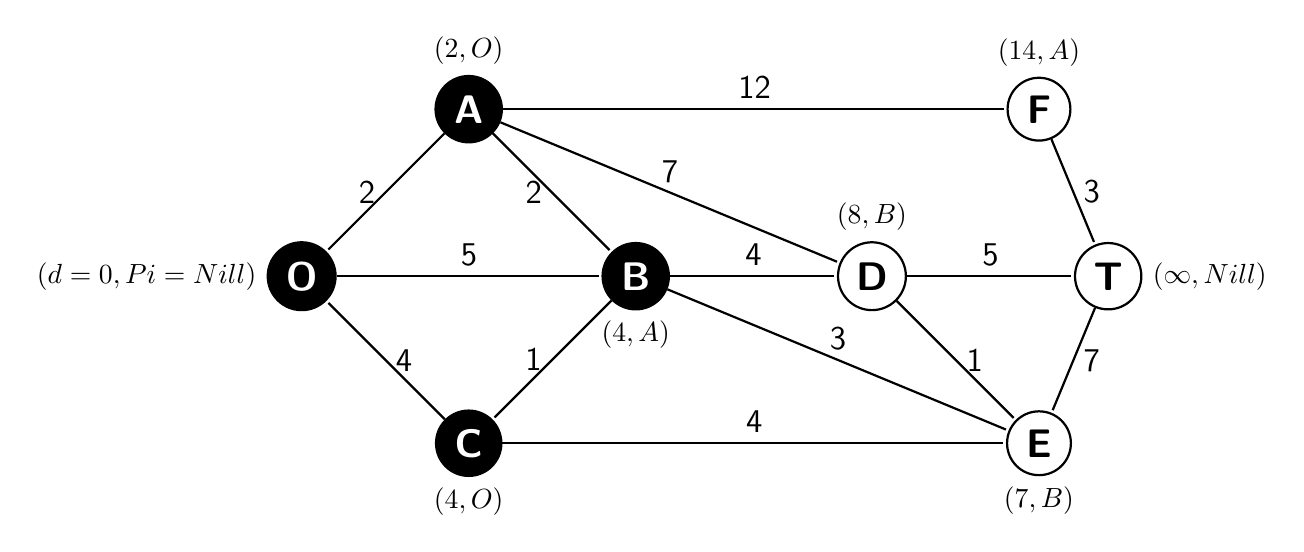
\begin{tikzpicture}[shorten >=1pt, auto, thick,
        node distance=3cm,
                    thick,main node/.style={circle,draw,font=\sffamily\Large\bfseries}]
                    
  %Any distance will not updated because it is already less than node + edge for all connected nodes
  
  \node[main node, fill={rgb,1:red,0; green,0; blue,0}, text=white, draw=black, label=above:{$(2,O)$}] (1) {A};
  \node[main node, fill={rgb,1:red,0; green,0; blue,0}, text=white, draw=black, label=left:{$(d=0,Pi=Nill)$}] (2) [below left of=1] {O};

  % Turning node C to black representing that C is visited
  \node[main node, fill={rgb,1:red,0; green,0; blue,0}, text=white, draw=black, label=below:{$(4,O)$}] (3) [below right of=2] {C};

  \node[main node, fill={rgb,1:red,0; green,0; blue,0}, text=white, draw=black, label=below:{$(4,A)$}] (4) [below right of=1] {B};
  
  %Setting distance of D and E by adding distance of C and edge weight
  \node[main node, label=above:{$(8,B)$}] (6) [right of=4] {D};
  \node[main node, label=above:{$(14,A)$}] (5) [above right of=6] {F};
  \node[main node, label=right:{$(\infty,Nill)$}] (7) [right of=6] {T};
  \node[main node, label=below:{$(7,B)$}] (8) [below right of=6] {E};

  \path[every node/.style={font=\sffamily\large}]
    (1) edge node [left] {2} (4)
        edge [right] node[left] {2} (2)
        edge [right] node[above] {12} (5)
        edge [right] node[above] {7} (6)
    (2) edge node {5} (4)
    (3) edge node [right] {4} (2)
        edge [right] node[above] {4} (8)
    (4) edge node [left] {1} (3)
        edge [right] node[above] {4} (6)
        edge [right] node[above] {3} (8)
    (5) edge node [right] {3} (7)
    (6) edge node [right] {1} (8)
        edge [right] node[above] {5} (7)
    (7) edge node [right] {7} (8);
\end{tikzpicture}

%Dijsktra's Traversal Step 5
\subsection*{Step 5:\newline}

%Graph
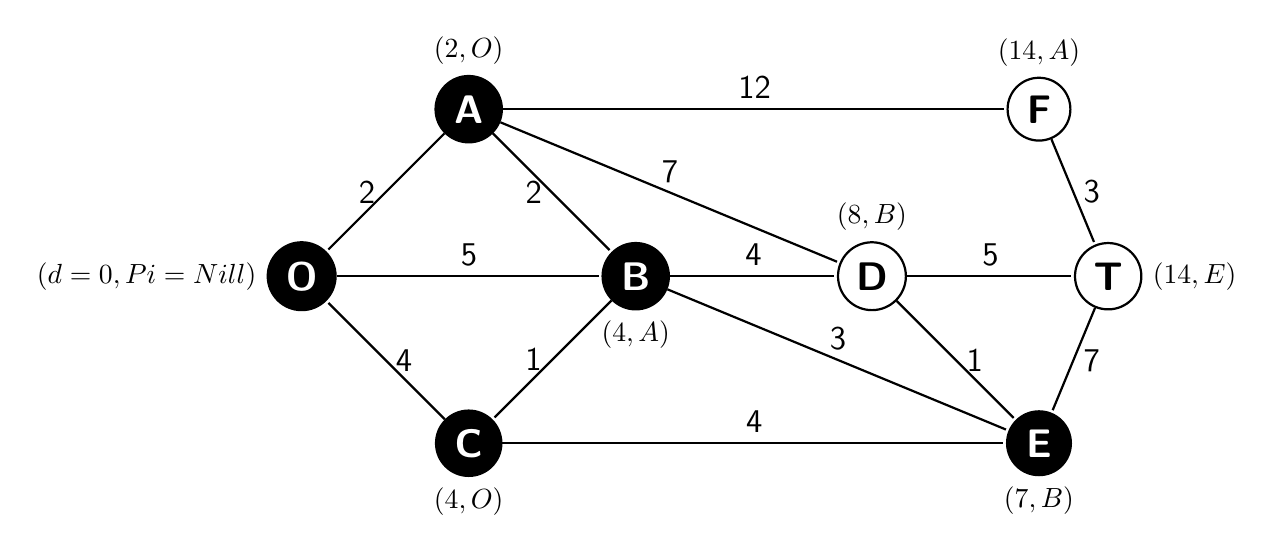
\begin{tikzpicture}[shorten >=1pt, auto, thick,
        node distance=3cm,
                    thick,main node/.style={circle,draw,font=\sffamily\Large\bfseries}]
                    
  %D distance will not updated because it is already equal to node + edge for all connected nodes
  
  \node[main node, fill={rgb,1:red,0; green,0; blue,0}, text=white, draw=black, label=above:{$(2,O)$}] (1) {A};
  \node[main node, fill={rgb,1:red,0; green,0; blue,0}, text=white, draw=black, label=left:{$(d=0,Pi=Nill)$}] (2) [below left of=1] {O};

  \node[main node, fill={rgb,1:red,0; green,0; blue,0}, text=white, draw=black, label=below:{$(4,O)$}] (3) [below right of=2] {C};

  \node[main node, fill={rgb,1:red,0; green,0; blue,0}, text=white, draw=black, label=below:{$(4,A)$}] (4) [below right of=1] {B};
  
  %Setting distance of T by adding distance of E and edge weight
  \node[main node, label=above:{$(8,B)$}] (6) [right of=4] {D};
  \node[main node, label=above:{$(14,A)$}] (5) [above right of=6] {F};
  \node[main node, label=right:{$(14,E)$}] (7) [right of=6] {T};
  
   % Turning node E to black representing that E is visited
  \node[main node, fill={rgb,1:red,0; green,0; blue,0}, text=white, draw=black, label=below:{$(7,B)$}] (8) [below right of=6] {E};

  \path[every node/.style={font=\sffamily\large}]
    (1) edge node [left] {2} (4)
        edge [right] node[left] {2} (2)
        edge [right] node[above] {12} (5)
        edge [right] node[above] {7} (6)
    (2) edge node {5} (4)
    (3) edge node [right] {4} (2)
        edge [right] node[above] {4} (8)
    (4) edge node [left] {1} (3)
        edge [right] node[above] {4} (6)
        edge [right] node[above] {3} (8)
    (5) edge node [right] {3} (7)
    (6) edge node [right] {1} (8)
        edge [right] node[above] {5} (7)
    (7) edge node [right] {7} (8);
\end{tikzpicture}


%Dijsktra's Traversal Step 6
\subsection*{Step 6:\newline}

%Graph
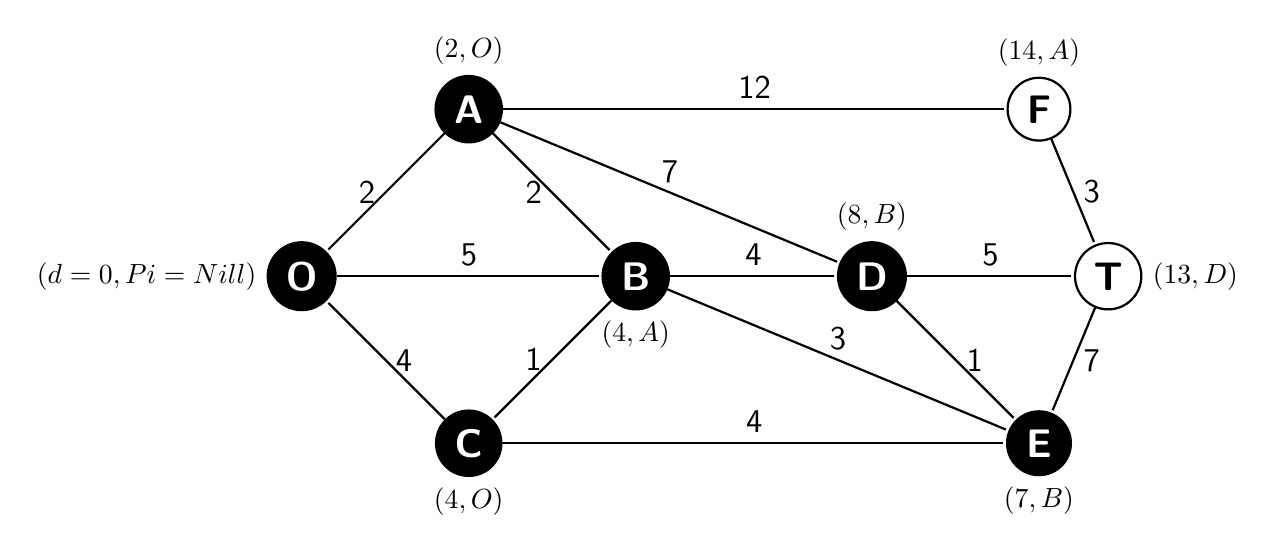
\begin{tikzpicture}[shorten >=1pt, auto, thick,
        node distance=3cm,
                    thick,main node/.style={circle,draw,font=\sffamily\Large\bfseries}]

  
  \node[main node, fill={rgb,1:red,0; green,0; blue,0}, text=white, draw=black, label=above:{$(2,O)$}] (1) {A};
  \node[main node, fill={rgb,1:red,0; green,0; blue,0}, text=white, draw=black, label=left:{$(d=0,Pi=Nill)$}] (2) [below left of=1] {O};

  \node[main node, fill={rgb,1:red,0; green,0; blue,0}, text=white, draw=black, label=below:{$(4,O)$}] (3) [below right of=2] {C};

  \node[main node, fill={rgb,1:red,0; green,0; blue,0}, text=white, draw=black, label=below:{$(4,A)$}] (4) [below right of=1] {B};

   % Turning node E to black representing that E is visited
  \node[main node, fill={rgb,1:red,0; green,0; blue,0}, text=white, draw=black, label=above:{$(8,B)$}] (6) [right of=4] {D};
  \node[main node, label=above:{$(14,A)$}] (5) [above right of=6] {F};  
  %Setting distance of T by adding distance of D and edge weight 
  \node[main node, label=right:{$(13,D)$}] (7) [right of=6] {T};
 
  \node[main node, fill={rgb,1:red,0; green,0; blue,0}, text=white, draw=black, label=below:{$(7,B)$}] (8) [below right of=6] {E};

  \path[every node/.style={font=\sffamily\large}]
    (1) edge node [left] {2} (4)
        edge [right] node[left] {2} (2)
        edge [right] node[above] {12} (5)
        edge [right] node[above] {7} (6)
    (2) edge node {5} (4)
    (3) edge node [right] {4} (2)
        edge [right] node[above] {4} (8)
    (4) edge node [left] {1} (3)
        edge [right] node[above] {4} (6)
        edge [right] node[above] {3} (8)
    (5) edge node [right] {3} (7)
    (6) edge node [right] {1} (8)
        edge [right] node[above] {5} (7)
    (7) edge node [right] {7} (8);
\end{tikzpicture}


%Dijsktra's Traversal Step 7
\subsection*{Step 7:\newline}

%Graph
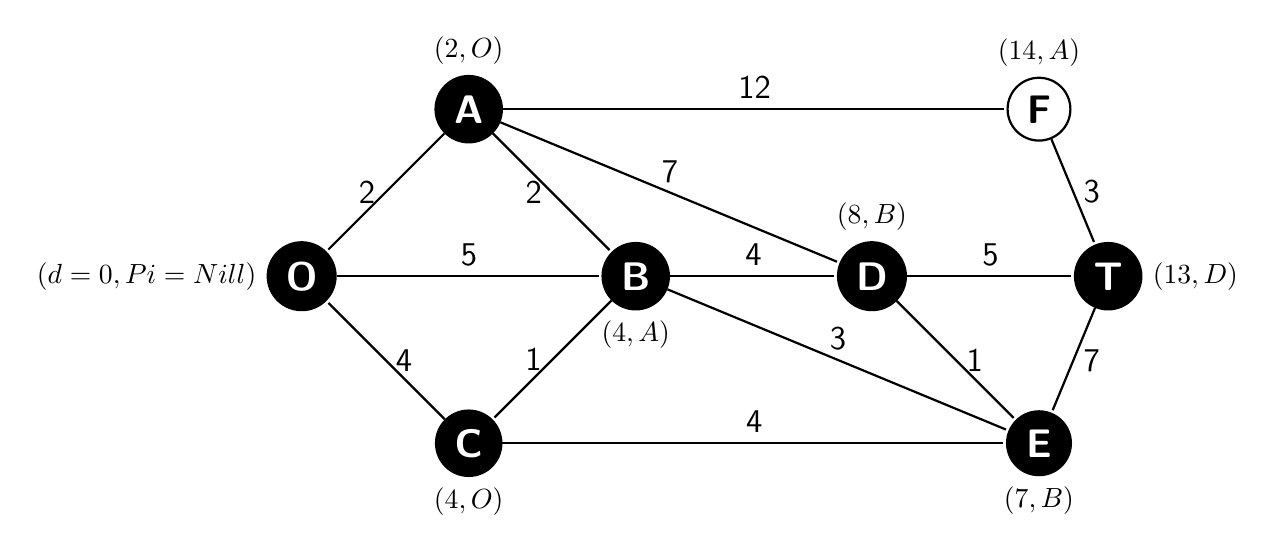
\begin{tikzpicture}[shorten >=1pt, auto, thick,
        node distance=3cm,
                    thick,main node/.style={circle,draw,font=\sffamily\Large\bfseries}]

  
  \node[main node, fill={rgb,1:red,0; green,0; blue,0}, text=white, draw=black, label=above:{$(2,O)$}] (1) {A};
  \node[main node, fill={rgb,1:red,0; green,0; blue,0}, text=white, draw=black, label=left:{$(d=0,Pi=Nill)$}] (2) [below left of=1] {O};

  \node[main node, fill={rgb,1:red,0; green,0; blue,0}, text=white, draw=black, label=below:{$(4,O)$}] (3) [below right of=2] {C};

  \node[main node, fill={rgb,1:red,0; green,0; blue,0}, text=white, draw=black, label=below:{$(4,A)$}] (4) [below right of=1] {B};


  \node[main node, fill={rgb,1:red,0; green,0; blue,0}, text=white, draw=black, label=above:{$(8,B)$}] (6) [right of=4] {D};
  \node[main node, label=above:{$(14,A)$}] (5) [above right of=6] {F};  
 
% Turning node T to black representing that T is visited
  \node[main node, fill={rgb,1:red,0; green,0; blue,0}, text=white, draw=black, label=right:{$(13,D)$}] (7) [right of=6] {T};
 
  \node[main node, fill={rgb,1:red,0; green,0; blue,0}, text=white, draw=black, label=below:{$(7,B)$}] (8) [below right of=6] {E};

  \path[every node/.style={font=\sffamily\large}]
    (1) edge node [left] {2} (4)
        edge [right] node[left] {2} (2)
        edge [right] node[above] {12} (5)
        edge [right] node[above] {7} (6)
    (2) edge node {5} (4)
    (3) edge node [right] {4} (2)
        edge [right] node[above] {4} (8)
    (4) edge node [left] {1} (3)
        edge [right] node[above] {4} (6)
        edge [right] node[above] {3} (8)
    (5) edge node [right] {3} (7)
    (6) edge node [right] {1} (8)
        edge [right] node[above] {5} (7)
    (7) edge node [right] {7} (8);
\end{tikzpicture}


%Dijsktra's Traversal Step 8
\subsection*{Step 8:\newline}

%Graph
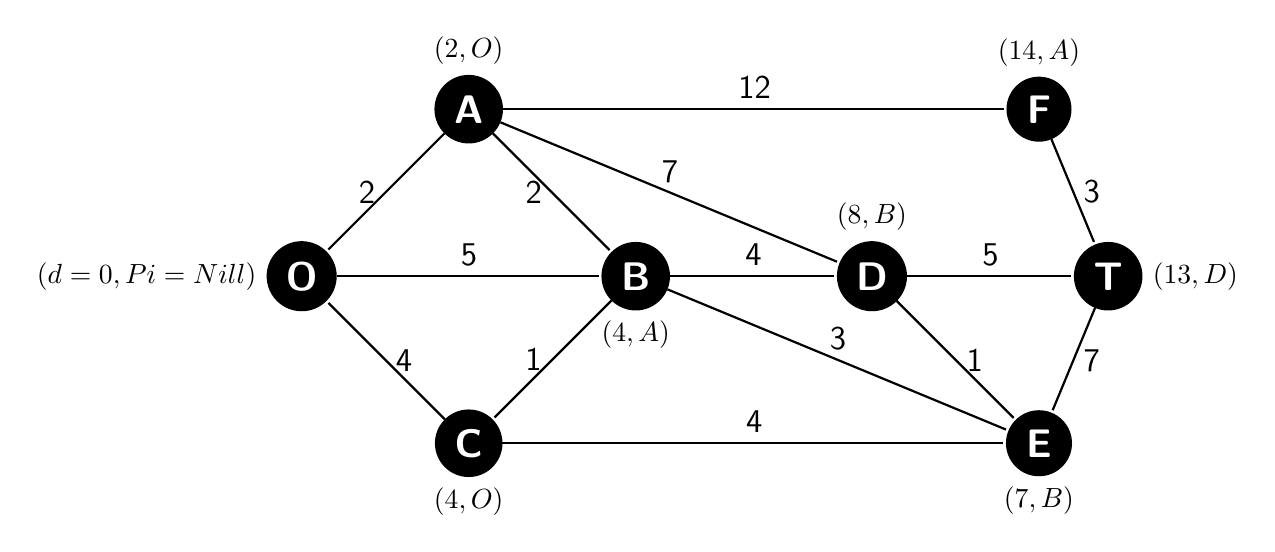
\begin{tikzpicture}[shorten >=1pt, auto, thick,
        node distance=3cm,
                    thick,main node/.style={circle,draw,font=\sffamily\Large\bfseries}]

  
  \node[main node, fill={rgb,1:red,0; green,0; blue,0}, text=white, draw=black, label=above:{$(2,O)$}] (1) {A};
  \node[main node, fill={rgb,1:red,0; green,0; blue,0}, text=white, draw=black, label=left:{$(d=0,Pi=Nill)$}] (2) [below left of=1] {O};

  \node[main node, fill={rgb,1:red,0; green,0; blue,0}, text=white, draw=black, label=below:{$(4,O)$}] (3) [below right of=2] {C};

  \node[main node, fill={rgb,1:red,0; green,0; blue,0}, text=white, draw=black, label=below:{$(4,A)$}] (4) [below right of=1] {B};


  \node[main node, fill={rgb,1:red,0; green,0; blue,0}, text=white, draw=black, label=above:{$(8,B)$}] (6) [right of=4] {D};
  \node[main node, fill={rgb,1:red,0; green,0; blue,0}, text=white, draw=black, label=above:{$(14,A)$}] (5) [above right of=6] {F};  
 
% Turning node F to black representing that F is visited
  \node[main node, fill={rgb,1:red,0; green,0; blue,0}, text=white, draw=black, label=right:{$(13,D)$}] (7) [right of=6] {T};
 
  \node[main node, fill={rgb,1:red,0; green,0; blue,0}, text=white, draw=black, label=below:{$(7,B)$}] (8) [below right of=6] {E};

  \path[every node/.style={font=\sffamily\large}]
    (1) edge node [left] {2} (4)
        edge [right] node[left] {2} (2)
        edge [right] node[above] {12} (5)
        edge [right] node[above] {7} (6)
    (2) edge node {5} (4)
    (3) edge node [right] {4} (2)
        edge [right] node[above] {4} (8)
    (4) edge node [left] {1} (3)
        edge [right] node[above] {4} (6)
        edge [right] node[above] {3} (8)
    (5) edge node [right] {3} (7)
    (6) edge node [right] {1} (8)
        edge [right] node[above] {5} (7)
    (7) edge node [right] {7} (8);
\end{tikzpicture}

\section*{\newline - Shortest Path from origin O to destination T}
\Large Shortest Distance from origin O to destination T is 13.\newline \newline
Path: \newline
$O \xrightarrow{} A \xrightarrow{} B \xrightarrow{} D \xrightarrow{} T$
\pagebreak


%Problem 2
\section*{\huge Problem 2}

%Problem statement

\large Let G = ( V, E, W ) be a connected graph, in which each edge weight we $\epsilon{}$ W, $\forall{}$ e $\epsilon{}$ E is distinct (i.e., not two edges have the same weight). Prove that G has a unique minimum spanning tree

\section{\huge Solution}
\large To prove that Graph G has a unique minimum spanning tree, we will use the cut property, which states that for any cut of the graph (i.e., a partition of the vertices into two disjoint sets), the minimum weight edge crossing the cut must be in the minimum spanning tree. Suppose for the sake of contradiction that G has two distinct minimum spanning trees, T1 and T2. Since T1 and T2 are both minimum-spanning trees, they must have the same weight which is the minimum of all. Now, let S be the set of vertices that are connected to vertex v by edges in T1 but not in T2, where v is any vertex in G. By the cut property, there must be a minimum weight edge e crossing the cut between S and the rest of the vertices in G. Since T1 is a minimum spanning tree, the weight of e must be less than or equal to the weight of any edge in T1 that crosses the same cut. However, since e is not in T2, another edge f in T2 must cross the same cut with the same weight. But we are given that no two edges have the same weight, so e and f cannot have the same weight. So we have to suppose that w(e) $<$ w(f). Then, we can replace f with e in T2 to obtain a new spanning tree T3 with a weight less than or equal to that of T2. Now, there are two cases:

\subsection*{Case 1:}
If T3 is a minimum spanning tree, then T1 and T3 have different weights, contradicting the assumption that T1 and T2 have the same weight.
\subsection*{Case 2:}
If T3 is not a minimum spanning tree, then there exists a spanning tree with a weight less than that of T3. But this contradicts the assumption that T1 and T2 are both minimum-spanning trees.

\section*{\large Conclusion:}
Thus, we have reached a contradiction in both cases, and so our assumption that G has two distinct minimum spanning trees must be false. Therefore, G has a unique minimum spanning tree.

\pagebreak

%Problem 3
\section*{\huge Problem 3}

%Problem statement

\Large Consider the Fibonacci heap on the right. Marked nodes are highlighted	in blue.\newline
\newline- Show the resulting heap after decrease-key(v,2).\newline
- Show the status of the heap after a subsequent extract-min operation.\newline \newline


%Graph
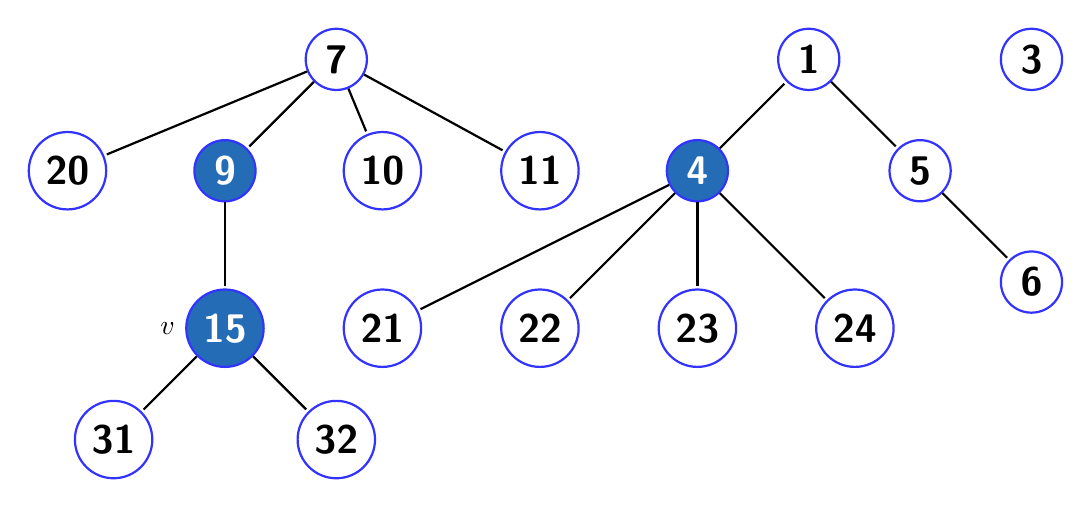
\begin{tikzpicture}[shorten >=1pt, auto, thick,
        node distance=2cm,
                    ,main node/.style={circle,draw=blue!80,font=\sffamily\Large\bfseries}]

  \node[main node] (1) {7};
  
  \node[main node] (2) [below left of=1, fill={rgb,70:red,10; green,30; blue,50}, text=white] {9};
  \node[main node] (3) [left of=2] {20};
  \node[main node] (4) [right of=2] {10};
  \node[main node] (5) [right of=4] {11};
  \node[main node, fill={rgb,70:red,10; green,30; blue,50}, text=white] (6) [below of=2, label=left:{$v$}] {15};
  \node[main node] (7) [below left of=6] {31};
  \node[main node] (8) [below right of=6] {32};

  \node[main node, fill={rgb,70:red,10; green,30; blue,50}, text=white] (9) [right of=5] {4};
  \node[main node] (10) [above right of=9] {1};
  \node[main node] (11) [below right of=10] {5};

  \node[main node] (12) [below of=4] {21};
  \node[main node] (13) [below of=5] {22};
  \node[main node] (14) [below of=9] {23};
  \node[main node] (15) [right of=14] {24};

  \node[main node] (16) [below right of=11] {6};
  \node[main node] (17) [above right of=11] {3};

  \path[every node/.style={font=\sffamily\large}]
    (1) edge node [left] {} (4)
        edge [right] node[left] {} (2)
        edge [right] node[above] {} (5)
        edge [right] node[above] {} (3)
    (2) edge node {} (6)
    (6) edge node [right] {} (8)
        edge [right] node[above] {} (7)
    (9) edge node [left] {} (12)
        edge node [right] {} (13)
        edge node [right] {} (14) 
        edge node [right] {} (15)
        edge node [right] {} (10)
    (10) edge node [left] {} (11)
    (11) edge node [left] {} (16);
\end{tikzpicture}

\section*{\huge Solution: }

\Large {- The	resulting	heap	after	decrease-key(v, 2)} \newline \newline

%Graph
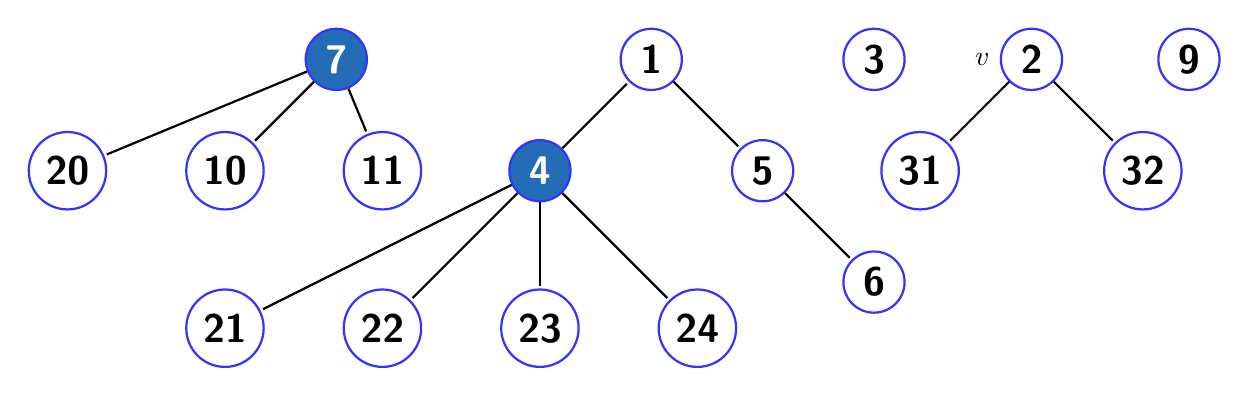
\begin{tikzpicture}[shorten >=1pt, auto, thick,
        node distance=2cm,
                    ,main node/.style={circle,draw=blue!80,font=\sffamily\Large\bfseries}]

  \node[main node, fill={rgb,70:red,10; green,30; blue,50}, text=white] (1) {7};

  \node[main node] (4) [below left of=1] {10};
  \node[main node] (3) [left of=4] {20};
  \node[main node] (5) [right of=4] {11};

  \node[main node, fill={rgb,70:red,10; green,30; blue,50}, text=white] (9) [right of=5] {4};
  \node[main node] (10) [above right of=9] {1};
  \node[main node] (11) [below right of=10] {5};

  \node[main node] (12) [below of=4] {21};
  \node[main node] (13) [below of=5] {22};
  \node[main node] (14) [below of=9] {23};
  \node[main node] (15) [right of=14] {24};

  \node[main node] (16) [below right of=11] {6};
  \node[main node] (17) [above right of=11] {3};

  \node[main node] (6) [right of=17, label=left:{$v$}] {2};
  \node[main node] (2) [right of=6] {9};
  
  \node[main node] (7) [below left of=6] {31};
  \node[main node] (8) [below right of=6] {32};

  \path[every node/.style={font=\sffamily\large}]
    (1) edge node [left] {} (4)
        edge [right] node[above] {} (5)
        edge [right] node[above] {} (3)
    (6) edge node [right] {} (8)
        edge [right] node[above] {} (7)
    (9) edge node [left] {} (12)
        edge node [right] {} (13)
        edge node [right] {} (14) 
        edge node [right] {} (15)
        edge node [right] {} (10)
    (10) edge node [left] {} (11)
    (11) edge node [left] {} (16);
\end{tikzpicture}

 
\Large {- The status of the heap after a subsequent extract-min operation.} \newline \newline

%Graph
\begin{tikzpicture}[shorten >=1pt, auto, thick,
        node distance=2cm,
                    ,main node/.style={circle,draw=blue!80,font=\sffamily\Large\bfseries}]

  \node[main node, fill={rgb,70:red,10; green,30; blue,50}, text=white] (9) [right of=5] {4};

  \node[main node] (12) [below of=4] {21};
  \node[main node] (6) [left of=12] {2};
  \node[main node] (13) [below of=5] {22};
  \node[main node] (14) [below of=9] {23};
  \node[main node] (15) [right of=14] {24};

  %\node[main node] (2) [right of=6] {9};
  
  \node[main node] (7) [below left of=6] {31};
  \node[main node] (17) [left of=7] {3};
  \node[main node] (11) [below left of=17] {5};
  \node[main node] (10) [right of=11] {9};
  \node[main node] (16) [below left of=11] {6};
  \node[main node] (8) [below right of=6] {32};
    \node[main node, fill={rgb,70:red,10; green,30; blue,50}, text=white] (1) [right of=8] {7};
  \node[main node] (4) [below left of=1] {10};
  \node[main node] (3) [left of=4] {20};
  \node[main node] (5) [right of=4] {11};

  \path[every node/.style={font=\sffamily\large}]
    (1) edge node [left] {} (4)
        edge [right] node[above] {} (5)
        edge [right] node[above] {} (3)
    (6) edge node [right] {} (8)
        edge [right] node[above] {} (7)
        edge [right] node[above] {} (17)
        edge [right] node[above] {} (1)
    (9) edge node [left] {} (12)
        edge node [right] {} (13)
        edge node [right] {} (14) 
        edge node [right] {} (15)
        edge node [left] {} (6)
    (11)edge node [left] {} (16)
    (17)edge node [left] {} (10)
        edge node [left] {} (11);
\end{tikzpicture}

\pagebreak


%Problem 4
\section*{\huge Problem 4}

%Problem statement
\Large  Suppose a minimum spanning tree(MST) has already been computed for a graph G using Kruskal’s algorithm. Let update-mst denote a procedure that updates	the	MST	when a new node (and its incident edges)is added to	G. Describe	update-mst and	derive its complexity

\section*{\huge Solution}
\large When a new node and its incident edges are added to a graph G for which a minimum spanning tree (MST) has already been computed using Kruskal's algorithm, we can update the MST using a procedure called Update-MST.\newline \newline
To perform Update-MST, we first add the new node and its incident edges to G.\newline \newline
We then initialize a set S containing the new node and all of its neighbors in G.\newline \newline
For each node v in S, we find the minimum-weight edge e=(v, w) connecting v to a node w in G-S, and add e to a priority queue Q. We then initialize an empty set A to store the new MST.
We then iterate through the priority queue Q while set A does not form a spanning tree. In each iteration, we remove the minimum-weight edge e=(v, w) from Q. If adding e to A creates a cycle, we discard e. Otherwise, we add e to A and add w to S.
The time complexity of Update-MST depends on the size of the graph and the number of edges added. Initializing Set takes O(d) time, where d is the degree of the new node. Making Priority Queue takes O(d log V) time, where V is the number of vertices in the graph. Iterating through Queue takes O(log V) time per iteration, and adding e to A takes O(d log V) time since we need to update the priority queue for each newly added node.\newline \newline
In total, the time complexity of the algorithm is O(E log V + d log V), where E is the number of edges in the graph. Note that if the number of edges added is much smaller than the total number of edges in the graph, then the time complexity can be reduced accordingly.

\pagebreak


%Problem 5
\section*{\huge Problem 5}

\Large  Consider the following algorithm to	compute	a topological	ordering of	a DAG. Recall that a topological ordering of	a graph is an ordering of its nodes	as v1,v2,...,vn so	that $\forall$ edge	(vi,vj)	we have	i >	j.

\section*{\huge Algorithm}
\large 1. Find	a node v with no incoming edges	and	order it first.\newline
2. Delete v	from graph G.\newline
3. Recursively	compute	a topological ordering of G	- {v} and append this	order after	v.\newline\
\setcounter{section}{1}
\subsection{}
\large Prove that this	algorithm does indeed result in	a topological	ordering of	G.

\section*{\Large Proof:}
\large We can prove the correctness of the given algorithm that it results in a topological ordering of G, by induction on the number of nodes in the DAG.\newline
\section*{\large Base case:}
If the DAG has only one node, then it has no incoming edges and the algorithm will correctly output the ordering
\section*{\large Inductive step:}
Let G be a DAG with n > 1 node, and assume that the algorithm correctly computes a topological ordering for any DAG with k nodes that is smaller than n.\newline

\large Let v be a node in G with no incoming edges. Since there are no incoming edges to v, it can be ordered first in any topological ordering of G.\newline

Now, let G' be the subgraph of G obtained by deleting v and all its outgoing edges. Since v has no outgoing edges, G' has n - 1 nodes. By the inductive hypothesis, the algorithm correctly computes a topological ordering of G', which we denote as v2, v3, ..., vn.\newline

We can append v to the beginning of this ordering to obtain a topological ordering of G as v, v2, v3, ..., vn.\newline

To see why this is a valid topological ordering, note that since v has no outgoing edges, it cannot be a successor of any other node in G, so there can be no edge (vi, v) for any i > 1. Furthermore, since v has no incoming edges, it cannot be a predecessor of any other node in G', so there can be no edge (v, vj) for any j < i. Therefore, the ordering v, v2, v3, ..., vn satisfies the condition that i < j whenever (vi, vj) is an edge in G.\newline

Therefore, the algorithm correctly computes a topological ordering of G, completing the inductive step and the proof.\newline

\subsection{}
\large Extend the given	algorithm for an arbitrary directed graph that may or may not be a DAG. Note: Your solution should take the form of a short essay. Specifically, a	topic paragraph should summarize the problem you are solving	and what your results are. The body	of the essay should	provide	
the	following:\newline
- A	description	of the algorithm in	English	and, if helpful, pseudo–code.\newline
- At least one	worked	example	or	diagram	to	show more precisely how your algorithm works.\newline
- A proof(or indication) of	the	correctness	of the algorithm.

\section*{\Large Proof:}
The problem we are solving is to extend the given algorithm for computing a topological ordering of a directed acyclic graph (DAG) to an arbitrary directed graph that may or may not be a DAG.\newline
In order to extend the algorithm, we need to handle the case where the graph contains cycles. If the graph contains a cycle, it cannot have a topological ordering since the ordering would need to violate the ordering constraint for at least one edge in the cycle. It means that the ordering will contain at least 1 back edge which is not permitted in the topological sortings. Therefore, our algorithm should detect cycles and report that the graph does not have a topological ordering if it contains any cycles.\newline


\section*{\large Extended Algorithm}
The extended algorithm can be described as follows:\newline
\newline 1.	Initialize a set S of vertices with no incoming edges.\newline
\newline 2.	Initialize a list L to store the topological ordering.\newline
\newline While S is not empty:\newline

     3. Remove a vertex v from S.\newline
     
     4. Append v to L.\newline
     
     5. For each node u such that there is an edge (v,u), remove the edge from the graph.\newline
     
     6. If u has no incoming edges after removing (v,u), add u to S.\newline
\newline 7. If there are still edges remaining in the graph, report that the graph contains a cycle and has no topological ordering.\newline
\newline 8. Otherwise, return the list L as the topological ordering.\newline

\section*{\large Working Example}

\large The algorithm works as follows: we start by initializing S to contain all nodes with no incoming edges. We then repeatedly remove a node v from S, append it to the topological ordering, and remove all outgoing edges from v. If any of these removals result in a node u having no incoming edges, we add u to S. If S is ever empty and there are still edges remaining in the graph, then the graph contains a cycle and we cannot have a topological ordering. Otherwise, we return the topological ordering as a list.
In pseudo-code, the algorithm looks like this:\newline \newline
\section*{\large Pseudo-code}
topological-sort(G):\newline
\newline S = set of nodes with no incoming edges\newline
\newline L = empty list for topological ordering\newline
\newline while S is not empty:\newline

remove a node v from S \newline

append v to L \newline

for each node u such that (v,u) is an edge in G: \newline

\quad remove the edge (v,u) from G \newline


\quad if u has no incoming edges: \newline


\qquad add u to S \newline
\newline if G still has edges:\newline

report that G contains a cycle and has no topological ordering\newline 
\newline else: \newline

return L\newline
\newline Overall, this extended algorithm can compute a topological ordering of an arbitrary directed graph if it exists and correctly reports if the graph contains a cycle and does not have a topological ordering

\section*{\huge Proof by Induction: }

To prove the correctness of the extended algorithm using induction, we need to show that the algorithm produces a valid topological ordering if one exists, and reports correctly if the graph contains a cycle and does not have a topological ordering.\newline

\section*{\Large Base case:}
\large If the graph has only one vertex, then it has no incoming edges and the algorithm will correctly output the ordering consisting of only that vertex.\newline

\section*{\Large Inductive step:}
\large Let G be a graph with n > 1 vertices, and assume that the algorithm correctly computes a topological ordering for any graph with fewer than n nodes.
If G has no cycles, then it is a DAG, and the algorithm will work as described for DAGs, producing a valid topological ordering.\newline

Now, assume that G contains at least one cycle. If the algorithm does not detect the cycle and reports a valid topological ordering, this must mean that the algorithm has incorrectly removed an edge in the cycle during one of the iterations, making it appear that the graph has no cycle. However, since the graph does contain a cycle, this is a contradiction, and therefore the algorithm must correctly detect the cycle and report that the graph does not have a topological ordering.\newline

Therefore, the algorithm correctly computes a topological ordering of G if one exists, and reports correctly if the graph contains a cycle and does not have a topological ordering. Hence, this is proved by induction that this algorithm is correct.\newline

\subsection{}
\large Provide an analysis of the running time of your algorithm.

\section*{\Large Time Complexity}
\large The execution time of the extended algorithm for computing the topological order of any directed graph is O(V + E).\newline

The main loop of the algorithm runs once for each node in the graph, removing a node from S, adding it to L, and removing all outgoing edges from that node at each iteration.\newline

The sum of degrees of all vertices in the graph is E, so the total time spent removing edges is O(E).\newline

For each removed edge, the algorithm checks the destination node for incoming edges.\newline

So the total time spent adding nodes to S is also O(E).
Checking the remaining edges takes O(E) time.\newline

So, as mentioned above, the total running time of the algorithm is O(V + E).

\pagebreak

%Problem 6
\section*{\huge Problem 6}

%Problem statement
\Large  Prove that for any directed graph G, the transpose of the component graph of GT is the same as the component graph of G

\section*{\huge Solution}
\subsection*{\huge Constructive Proof:}
\large To prove that the component graph transpose GT is the same as the component graph of any directed graph G, we must show that these two graphs have the same vertices and edges.
The component graph of a directed graph G is such that the nodes represent the strongly connected components (SCCs) of G and the edges from any one node of the first SCC to any one node of the second SCC.\newline


When considering the transpose of the component graph of GT, it is important to note that this graph has the same vertices as the component graph of G since the vertices of GT are equivalent to the vertices of G. However, it must also be shown that these graphs have the same edges.\newline


If an edge from SCC 1 to SCC 2 exists in the component graph of G, this implies that there is at least one edge in G from anyone node in SCC 1 to a node in SCC 2. Since GT is the transpose of G, there must be at least one edge from a node in SCC 2 of GT to a node in SCC 2. Thus, in the transpose of the component graph of G, there exists an edge from SCC 2 to SCC 1.\newline


Conversely, if there is an edge from SCC 1 to SCC 2 in the transpose of GT's component graph, this means that there is at least one edge from GT's node of his SCC 2 to the node of SCC 1. means Since GT is the transpose of G, this means that there is at least one edge in G from a node in SCC 1 to a node in SCC 2. Therefore, the component graph of G has an edge from SCC 1 to SCC 2. Having shown that two graphs share the same vertices and edges, we can conclude that the component graph transpose of GT is the same as the component graph transpose of any directed graph G.\newline


To prove that the component graph transpose GT is the same as the component graph of any directed graph G, we must show that these two graphs have the same vertices and edges.
The component graph of a directed graph G is such that the nodes represent the strongly connected components (SCCs) of G and the edges from any one node of the first SCC to any one node of the second SCC.\newline


When considering the transpose of the component graph of GT, it is important to note that this graph has the same vertices as the component graph of G since the vertices of GT are equivalent to the vertices of G. However, it must also be shown that these graphs have the same edges.\newline


If an edge from SCC 1 to SCC 2 exists in the component graph of G, this implies that there is at least one edge in G from anyone node in SCC 1 to a node in SCC 2. Since GT is the transpose of G, there must be at least one edge from a node in SCC 2 of GT to a node in SCC 2. Thus, in the transpose of the component graph of G, there exists an edge from SCC 2 to SCC 1.\newline


Conversely, if there is an edge from SCC 1 to SCC 2 in the transpose of GT's component graph, this means that there is at least one edge from GT's node of his SCC 2 to the node of SCC 1. means Since GT is the transpose of G, this means that there is at least one edge in G from a node in SCC 1 to a node in SCC 2. Therefore, the component graph of G has an edge from SCC 1 to SCC 2. Having shown that two graphs share the same vertices and edges, we can conclude that the component graph transpose of GT is the same as the component graph transpose of any directed graph G.\newline

\subsection*{\huge Proof by Contradiction:}

\large Assume that for a directed graph G, the transpose of the component graph of GT is not the same as the component graph of G.\newline


This means that there exists at least one node or edge in one graph that is not present in the other graph.
Let's consider the case where there exists a node in the component graph of G that is not present in the transpose of the component graph of GT.\newline


Since the nodes in the component graph of G represent strongly connected components of G, this means that there is at least one SCC in G that is not strongly connected in GT.
However, by definition of the transpose of a graph, if there exists an edge from node u to node v in G, then there exists an edge from node v to node u in GT.\newline


This means that if there is an SCC in G that is not strongly connected in GT, then there must be at least one edge in G that is not present in GT.\newline


But this contradicts the assumption that the transpose of the component graph of GT is not the same as the component graph of G.\newline


Therefore, our initial assumption must be false, and we can conclude that for any directed graph G, the transpose of the component graph of GT is the same as the component graph of G.\newline


Assume that for a directed graph G, the transpose of the component graph of GT is not the same as the component graph of G.\newline


This means that there exists at least one node or edge in one graph that is not present in the other graph.\newline


Let's consider the case where there exists a node in the component graph of G that is not present in the transpose of the component graph of GT.\newline


Since the nodes in the component graph of G represent strongly connected components of G, this means that there is at least one SCC in G that is not strongly connected in GT.\newline


However, by definition of the transpose of a graph, if there exists an edge from node u to node v in G, then there exists an edge from node v to node u in GT.\newline


This means that if there is an SCC in G that is not strongly connected in GT, then there must be at least one edge in G that is not present in GT.\newline


But this contradicts the assumption that the transpose of the component graph of GT is not the same as the component graph of G.\newline


Therefore, our initial assumption must be false, and we can conclude that for any directed graph G, the transpose of the component graph of GT is the same as the component graph of G.\newline
\end{document}

